% Options for packages loaded elsewhere
\PassOptionsToPackage{unicode}{hyperref}
\PassOptionsToPackage{hyphens}{url}
\PassOptionsToPackage{dvipsnames,svgnames,x11names}{xcolor}
%
\documentclass[
  letterpaper,
  DIV=11,
  numbers=noendperiod]{scrreprt}

\usepackage{amsmath,amssymb}
\usepackage{iftex}
\ifPDFTeX
  \usepackage[T1]{fontenc}
  \usepackage[utf8]{inputenc}
  \usepackage{textcomp} % provide euro and other symbols
\else % if luatex or xetex
  \usepackage{unicode-math}
  \defaultfontfeatures{Scale=MatchLowercase}
  \defaultfontfeatures[\rmfamily]{Ligatures=TeX,Scale=1}
\fi
\usepackage{lmodern}
\ifPDFTeX\else  
    % xetex/luatex font selection
\fi
% Use upquote if available, for straight quotes in verbatim environments
\IfFileExists{upquote.sty}{\usepackage{upquote}}{}
\IfFileExists{microtype.sty}{% use microtype if available
  \usepackage[]{microtype}
  \UseMicrotypeSet[protrusion]{basicmath} % disable protrusion for tt fonts
}{}
\makeatletter
\@ifundefined{KOMAClassName}{% if non-KOMA class
  \IfFileExists{parskip.sty}{%
    \usepackage{parskip}
  }{% else
    \setlength{\parindent}{0pt}
    \setlength{\parskip}{6pt plus 2pt minus 1pt}}
}{% if KOMA class
  \KOMAoptions{parskip=half}}
\makeatother
\usepackage{xcolor}
\setlength{\emergencystretch}{3em} % prevent overfull lines
\setcounter{secnumdepth}{5}
% Make \paragraph and \subparagraph free-standing
\ifx\paragraph\undefined\else
  \let\oldparagraph\paragraph
  \renewcommand{\paragraph}[1]{\oldparagraph{#1}\mbox{}}
\fi
\ifx\subparagraph\undefined\else
  \let\oldsubparagraph\subparagraph
  \renewcommand{\subparagraph}[1]{\oldsubparagraph{#1}\mbox{}}
\fi

\usepackage{color}
\usepackage{fancyvrb}
\newcommand{\VerbBar}{|}
\newcommand{\VERB}{\Verb[commandchars=\\\{\}]}
\DefineVerbatimEnvironment{Highlighting}{Verbatim}{commandchars=\\\{\}}
% Add ',fontsize=\small' for more characters per line
\usepackage{framed}
\definecolor{shadecolor}{RGB}{241,243,245}
\newenvironment{Shaded}{\begin{snugshade}}{\end{snugshade}}
\newcommand{\AlertTok}[1]{\textcolor[rgb]{0.68,0.00,0.00}{#1}}
\newcommand{\AnnotationTok}[1]{\textcolor[rgb]{0.37,0.37,0.37}{#1}}
\newcommand{\AttributeTok}[1]{\textcolor[rgb]{0.40,0.45,0.13}{#1}}
\newcommand{\BaseNTok}[1]{\textcolor[rgb]{0.68,0.00,0.00}{#1}}
\newcommand{\BuiltInTok}[1]{\textcolor[rgb]{0.00,0.23,0.31}{#1}}
\newcommand{\CharTok}[1]{\textcolor[rgb]{0.13,0.47,0.30}{#1}}
\newcommand{\CommentTok}[1]{\textcolor[rgb]{0.37,0.37,0.37}{#1}}
\newcommand{\CommentVarTok}[1]{\textcolor[rgb]{0.37,0.37,0.37}{\textit{#1}}}
\newcommand{\ConstantTok}[1]{\textcolor[rgb]{0.56,0.35,0.01}{#1}}
\newcommand{\ControlFlowTok}[1]{\textcolor[rgb]{0.00,0.23,0.31}{#1}}
\newcommand{\DataTypeTok}[1]{\textcolor[rgb]{0.68,0.00,0.00}{#1}}
\newcommand{\DecValTok}[1]{\textcolor[rgb]{0.68,0.00,0.00}{#1}}
\newcommand{\DocumentationTok}[1]{\textcolor[rgb]{0.37,0.37,0.37}{\textit{#1}}}
\newcommand{\ErrorTok}[1]{\textcolor[rgb]{0.68,0.00,0.00}{#1}}
\newcommand{\ExtensionTok}[1]{\textcolor[rgb]{0.00,0.23,0.31}{#1}}
\newcommand{\FloatTok}[1]{\textcolor[rgb]{0.68,0.00,0.00}{#1}}
\newcommand{\FunctionTok}[1]{\textcolor[rgb]{0.28,0.35,0.67}{#1}}
\newcommand{\ImportTok}[1]{\textcolor[rgb]{0.00,0.46,0.62}{#1}}
\newcommand{\InformationTok}[1]{\textcolor[rgb]{0.37,0.37,0.37}{#1}}
\newcommand{\KeywordTok}[1]{\textcolor[rgb]{0.00,0.23,0.31}{#1}}
\newcommand{\NormalTok}[1]{\textcolor[rgb]{0.00,0.23,0.31}{#1}}
\newcommand{\OperatorTok}[1]{\textcolor[rgb]{0.37,0.37,0.37}{#1}}
\newcommand{\OtherTok}[1]{\textcolor[rgb]{0.00,0.23,0.31}{#1}}
\newcommand{\PreprocessorTok}[1]{\textcolor[rgb]{0.68,0.00,0.00}{#1}}
\newcommand{\RegionMarkerTok}[1]{\textcolor[rgb]{0.00,0.23,0.31}{#1}}
\newcommand{\SpecialCharTok}[1]{\textcolor[rgb]{0.37,0.37,0.37}{#1}}
\newcommand{\SpecialStringTok}[1]{\textcolor[rgb]{0.13,0.47,0.30}{#1}}
\newcommand{\StringTok}[1]{\textcolor[rgb]{0.13,0.47,0.30}{#1}}
\newcommand{\VariableTok}[1]{\textcolor[rgb]{0.07,0.07,0.07}{#1}}
\newcommand{\VerbatimStringTok}[1]{\textcolor[rgb]{0.13,0.47,0.30}{#1}}
\newcommand{\WarningTok}[1]{\textcolor[rgb]{0.37,0.37,0.37}{\textit{#1}}}

\providecommand{\tightlist}{%
  \setlength{\itemsep}{0pt}\setlength{\parskip}{0pt}}\usepackage{longtable,booktabs,array}
\usepackage{calc} % for calculating minipage widths
% Correct order of tables after \paragraph or \subparagraph
\usepackage{etoolbox}
\makeatletter
\patchcmd\longtable{\par}{\if@noskipsec\mbox{}\fi\par}{}{}
\makeatother
% Allow footnotes in longtable head/foot
\IfFileExists{footnotehyper.sty}{\usepackage{footnotehyper}}{\usepackage{footnote}}
\makesavenoteenv{longtable}
\usepackage{graphicx}
\makeatletter
\def\maxwidth{\ifdim\Gin@nat@width>\linewidth\linewidth\else\Gin@nat@width\fi}
\def\maxheight{\ifdim\Gin@nat@height>\textheight\textheight\else\Gin@nat@height\fi}
\makeatother
% Scale images if necessary, so that they will not overflow the page
% margins by default, and it is still possible to overwrite the defaults
% using explicit options in \includegraphics[width, height, ...]{}
\setkeys{Gin}{width=\maxwidth,height=\maxheight,keepaspectratio}
% Set default figure placement to htbp
\makeatletter
\def\fps@figure{htbp}
\makeatother
% definitions for citeproc citations
\NewDocumentCommand\citeproctext{}{}
\NewDocumentCommand\citeproc{mm}{%
  \begingroup\def\citeproctext{#2}\cite{#1}\endgroup}
\makeatletter
 % allow citations to break across lines
 \let\@cite@ofmt\@firstofone
 % avoid brackets around text for \cite:
 \def\@biblabel#1{}
 \def\@cite#1#2{{#1\if@tempswa , #2\fi}}
\makeatother
\newlength{\cslhangindent}
\setlength{\cslhangindent}{1.5em}
\newlength{\csllabelwidth}
\setlength{\csllabelwidth}{3em}
\newenvironment{CSLReferences}[2] % #1 hanging-indent, #2 entry-spacing
 {\begin{list}{}{%
  \setlength{\itemindent}{0pt}
  \setlength{\leftmargin}{0pt}
  \setlength{\parsep}{0pt}
  % turn on hanging indent if param 1 is 1
  \ifodd #1
   \setlength{\leftmargin}{\cslhangindent}
   \setlength{\itemindent}{-1\cslhangindent}
  \fi
  % set entry spacing
  \setlength{\itemsep}{#2\baselineskip}}}
 {\end{list}}
\usepackage{calc}
\newcommand{\CSLBlock}[1]{\hfill\break\parbox[t]{\linewidth}{\strut\ignorespaces#1\strut}}
\newcommand{\CSLLeftMargin}[1]{\parbox[t]{\csllabelwidth}{\strut#1\strut}}
\newcommand{\CSLRightInline}[1]{\parbox[t]{\linewidth - \csllabelwidth}{\strut#1\strut}}
\newcommand{\CSLIndent}[1]{\hspace{\cslhangindent}#1}

\KOMAoption{captions}{tableheading}
\makeatletter
\@ifpackageloaded{tcolorbox}{}{\usepackage[skins,breakable]{tcolorbox}}
\@ifpackageloaded{fontawesome5}{}{\usepackage{fontawesome5}}
\definecolor{quarto-callout-color}{HTML}{909090}
\definecolor{quarto-callout-note-color}{HTML}{0758E5}
\definecolor{quarto-callout-important-color}{HTML}{CC1914}
\definecolor{quarto-callout-warning-color}{HTML}{EB9113}
\definecolor{quarto-callout-tip-color}{HTML}{00A047}
\definecolor{quarto-callout-caution-color}{HTML}{FC5300}
\definecolor{quarto-callout-color-frame}{HTML}{acacac}
\definecolor{quarto-callout-note-color-frame}{HTML}{4582ec}
\definecolor{quarto-callout-important-color-frame}{HTML}{d9534f}
\definecolor{quarto-callout-warning-color-frame}{HTML}{f0ad4e}
\definecolor{quarto-callout-tip-color-frame}{HTML}{02b875}
\definecolor{quarto-callout-caution-color-frame}{HTML}{fd7e14}
\makeatother
\makeatletter
\@ifpackageloaded{bookmark}{}{\usepackage{bookmark}}
\makeatother
\makeatletter
\@ifpackageloaded{caption}{}{\usepackage{caption}}
\AtBeginDocument{%
\ifdefined\contentsname
  \renewcommand*\contentsname{Table of contents}
\else
  \newcommand\contentsname{Table of contents}
\fi
\ifdefined\listfigurename
  \renewcommand*\listfigurename{List of Figures}
\else
  \newcommand\listfigurename{List of Figures}
\fi
\ifdefined\listtablename
  \renewcommand*\listtablename{List of Tables}
\else
  \newcommand\listtablename{List of Tables}
\fi
\ifdefined\figurename
  \renewcommand*\figurename{Figure}
\else
  \newcommand\figurename{Figure}
\fi
\ifdefined\tablename
  \renewcommand*\tablename{Table}
\else
  \newcommand\tablename{Table}
\fi
}
\@ifpackageloaded{float}{}{\usepackage{float}}
\floatstyle{ruled}
\@ifundefined{c@chapter}{\newfloat{codelisting}{h}{lop}}{\newfloat{codelisting}{h}{lop}[chapter]}
\floatname{codelisting}{Listing}
\newcommand*\listoflistings{\listof{codelisting}{List of Listings}}
\makeatother
\makeatletter
\makeatother
\makeatletter
\@ifpackageloaded{caption}{}{\usepackage{caption}}
\@ifpackageloaded{subcaption}{}{\usepackage{subcaption}}
\makeatother
\ifLuaTeX
  \usepackage{selnolig}  % disable illegal ligatures
\fi
\usepackage{bookmark}

\IfFileExists{xurl.sty}{\usepackage{xurl}}{} % add URL line breaks if available
\urlstyle{same} % disable monospaced font for URLs
\hypersetup{
  pdftitle={User Guide: Implementation of Imputation Likelihood Methods in Estimating Missing Data Values in R},
  pdfauthor={Tyler Davis},
  colorlinks=true,
  linkcolor={blue},
  filecolor={Maroon},
  citecolor={Blue},
  urlcolor={Blue},
  pdfcreator={LaTeX via pandoc}}

\title{User Guide: Implementation of Imputation Likelihood Methods in
Estimating Missing Data Values in R}
\author{Tyler Davis}
\date{March 13, 2025}

\begin{document}
\maketitle

\renewcommand*\contentsname{Table of contents}
{
\hypersetup{linkcolor=}
\setcounter{tocdepth}{2}
\tableofcontents
}
\bookmarksetup{startatroot}

\chapter*{Assignment Flow}\label{assignment-flow}
\addcontentsline{toc}{chapter}{Assignment Flow}

\markboth{Assignment Flow}{Assignment Flow}

This project is set up to scaffold this user guide and set you up for
success.

Start at \texttt{topic.qmd} and identify a topic for your user guide.

Once you've proposed a topic and received my approval/feedback, you can
convert the contents of \texttt{topic.qmd} into an introductory
paragraph in your report. Please leave the \texttt{topic.qmd} file as an
appendix, to document the different stages of this project.

Once we've agreed on a topic for your user guide, you will proceed to
\texttt{needs.qmd} and \texttt{task-analysis.qmd}. Both will be
submitted at the same check-in, and both will be included in your final
report as appendices. You should be able to re-purpose most of the
information in \texttt{task-analysis.qmd} to orient the user to
different components of the task you've chosen.

Your next step is to actually write the content that satisfies the work
you outlined in \texttt{task-analysis.qmd}.

Once you're finished with that, ideally, you'll have plenty of time to
edit and streamline your report. Feel free to trade reports with a
friend and try to complete your friend's task - this will help you both
identify areas where the guide isn't as clear. Try to complete the task
with a different data set - that often helps find trouble spots.

When you submit your final report, you may remove \texttt{index.qmd}
from the \texttt{\_quarto.yml} file, which will remove this chapter
(which is quite unnecessary for your user) from the report. You should
also take the time to make sure your name is listed as both author and
copyright holder in the \texttt{\_quarto.yml} file. Feel free to make a
custom cover for your manual if you would like to do so. You can also
tweak the CSS/theme for the book, so long as you're conscious of
accessibility concerns.

\begin{tcolorbox}[enhanced jigsaw, colframe=quarto-callout-caution-color-frame, breakable, opacityback=0, toprule=.15mm, rightrule=.15mm, bottomtitle=1mm, title=\textcolor{quarto-callout-caution-color}{\faFire}\hspace{0.5em}{Building the report}, left=2mm, toptitle=1mm, titlerule=0mm, opacitybacktitle=0.6, colbacktitle=quarto-callout-caution-color!10!white, coltitle=black, arc=.35mm, leftrule=.75mm, bottomrule=.15mm, colback=white]

If you are using RStudio to complete this report, you can hit
(Ctrl/Cmd)-Shift-B to build the whole report. You can also type
\texttt{quarto\ render\ .} on the command line in the project folder to
accomplish the same thing.

If you have questions about how to customize or debug your book, it may
be helpful to start at the quarto book documentation (Posit PBC 2024).

\end{tcolorbox}

\bookmarksetup{startatroot}

\chapter{Introduction}\label{introduction}

Data has become the lifeblood on today's world. It is used in almost
every industry to track, organize, and solve businesses problems. This
is why it is more crucial than ever to understand how to handle data
properly to get results that can help you grow your business. One of the
issues that comes across when analyzing a data set in dealing with
missing values. Our first instinct is to throw those values out and
analyze that data that we do have, yet this is not a viable option
according to Little, Little (2021). Little discusses in his paper a
variety of ways to properly estimate missing values in a data set, one
option is imputation likelihood methods. This method allows you to get
estimates for your missing values which intern allows you to get
accurate information from your data set as a whole. A package called
``mice'' found in R can complete these missing data estimations which
allow you to properly analyze your data, Van Buuren and
Groothuis-Oudshoorn (n.d.). This guide will attempt to discuss the
processes and methods involved with using this package on a data set.
This example will be used as a guide to understanding how to implement
this package on future data that you may come across.

\section{Prerequisites}\label{prerequisites}

The prerequisites to understanding how to use this package are basic
statistical knowledge and ability on par with running a linear model in
R. You have to understand how to recognize missing data and how to
classify variables, numerical, categorical, etc. Knowing what missing
data is. You must understand the basics of matrices along with applying
different manipulations to data. The software needed to complete this
task can be found in the R packages lattice and mice for the simple
example which will be described in detail below. There is other packages
that the you may need but that will be on a case by case basis.

\section{Explanation of Example}\label{explanation-of-example}

\subsection{Motivation}\label{motivation}

The example from the mice package will show the basics of how and when
to use this package to estimate missing values in a data set. This will
allow you to have a basis of understanding regarding estimation of
missing values using the mice package.

\subsection{Example}\label{example}

\begin{enumerate}
\def\labelenumi{\arabic{enumi}.}
\tightlist
\item
  The first step of this example is to load in the mice package. The
  next object is to load in an example data set from the mice package
  for demonstration. In most cases your data set will be loaded in
  before you call you package. This will allow you to see the structure
  of the data and if the mice package is necessary.
\end{enumerate}

\begin{Shaded}
\begin{Highlighting}[]
\CommentTok{\# Load required package}
\FunctionTok{library}\NormalTok{(mice)}
\end{Highlighting}
\end{Shaded}

\begin{verbatim}
Warning: package 'mice' was built under R version 4.3.3
\end{verbatim}

\begin{verbatim}
Warning in check_dep_version(): ABI version mismatch: 
lme4 was built with Matrix ABI version 1
Current Matrix ABI version is 0
Please re-install lme4 from source or restore original 'Matrix' package
\end{verbatim}

\begin{verbatim}

Attaching package: 'mice'
\end{verbatim}

\begin{verbatim}
The following object is masked from 'package:stats':

    filter
\end{verbatim}

\begin{verbatim}
The following objects are masked from 'package:base':

    cbind, rbind
\end{verbatim}

\begin{Shaded}
\begin{Highlighting}[]
\CommentTok{\# Load example dataset}
\FunctionTok{data}\NormalTok{(nhanes2)}
\FunctionTok{head}\NormalTok{(nhanes2)}
\end{Highlighting}
\end{Shaded}

\begin{verbatim}
    age  bmi  hyp chl
1 20-39   NA <NA>  NA
2 40-59 22.7   no 187
3 20-39   NA   no 187
4 60-99   NA <NA>  NA
5 20-39 20.4   no 113
6 60-99   NA <NA> 184
\end{verbatim}

\begin{Shaded}
\begin{Highlighting}[]
\CommentTok{\# Check the structure of the dataset}
\FunctionTok{str}\NormalTok{(nhanes2)}
\end{Highlighting}
\end{Shaded}

\begin{verbatim}
'data.frame':   25 obs. of  4 variables:
 $ age: Factor w/ 3 levels "20-39","40-59",..: 1 2 1 3 1 3 1 1 2 2 ...
 $ bmi: num  NA 22.7 NA NA 20.4 NA 22.5 30.1 22 NA ...
 $ hyp: Factor w/ 2 levels "no","yes": NA 1 1 NA 1 NA 1 1 1 NA ...
 $ chl: num  NA 187 187 NA 113 184 118 187 238 NA ...
\end{verbatim}

We can see from the output provided we can see that type of variables we
are dealing with along with what they will be coded as in the data set.
We can see that we have 25 observations with 4 variables. We can also
see the type of each variable which will come in handy later when
selecting the imputation method to estimate the missing values.

\begin{enumerate}
\def\labelenumi{\arabic{enumi}.}
\setcounter{enumi}{1}
\item
  The next step is optional and it is to create a plot that will allow
  you to see where the missing values are in your data set.

\begin{Shaded}
\begin{Highlighting}[]
\CommentTok{\# Check missing data pattern}
\FunctionTok{md.pattern}\NormalTok{(nhanes2)}
\end{Highlighting}
\end{Shaded}

  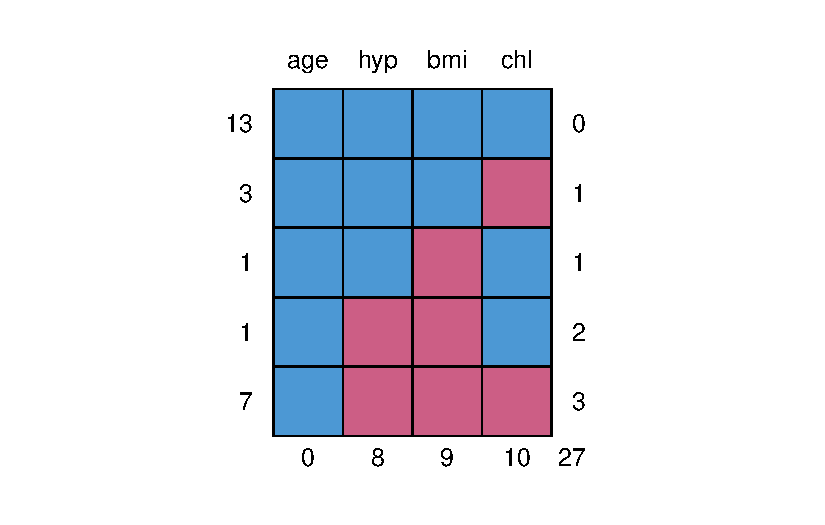
\includegraphics{guide_files/figure-pdf/unnamed-chunk-2-1.pdf}

\begin{verbatim}
   age hyp bmi chl   
13   1   1   1   1  0
3    1   1   1   0  1
1    1   1   0   1  1
1    1   0   0   1  2
7    1   0   0   0  3
     0   8   9  10 27
\end{verbatim}
\end{enumerate}

This graph shows us the pattern of missingness between variables. This
plot can be broken down into different parts, the bottom row tells you
how many missing values are in each variable. The red boxes show missing
values while blue boxes show non - missing values. The left hand column
shows the number of rows that follow the missingness pattern, while the
right hand column shows the number of missing values in each row. This
graph gives us a visual description of the data and the mssingness
pattern throughout. You can make this graph to deepen your understanding
of the missingness patterns in your data which paint a better picture
than just the structure of the data.

\begin{enumerate}
\def\labelenumi{\arabic{enumi}.}
\setcounter{enumi}{2}
\item
  You now understand the missingness pattern in the data you must now
  apply methods of estimations for the mice package. You can do this by
  understanding how each variable is categorized. We can look back at
  the structure of the data found in step 1. This will allow us to see
  how to apply methods of estimation as it is based on the type of
  variables you are dealing with.

  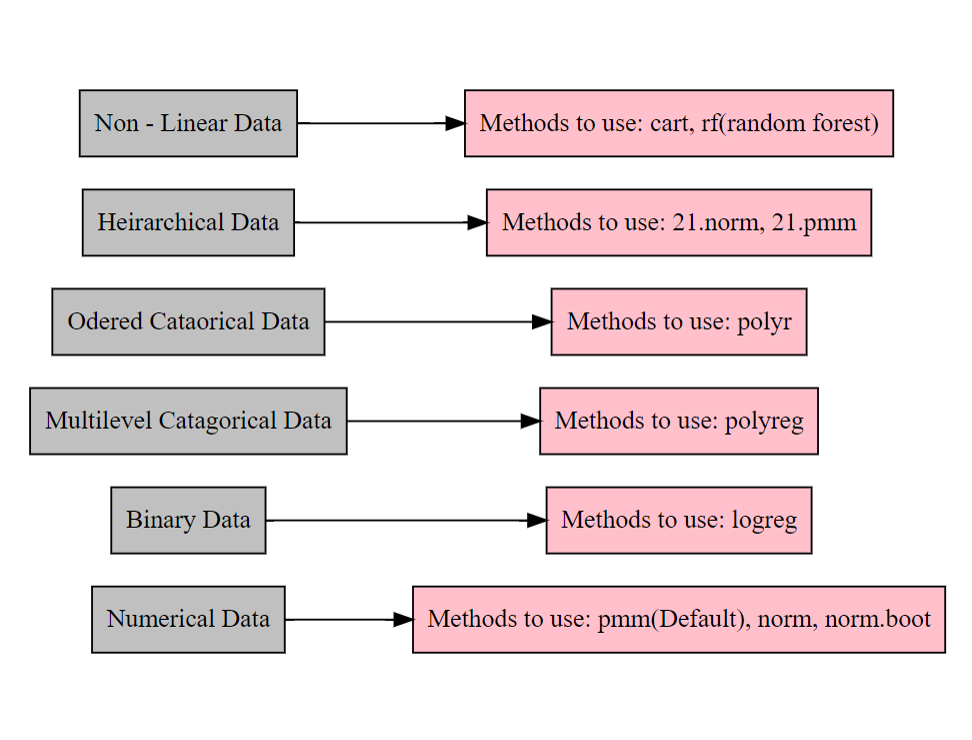
\includegraphics{flow chart.png}
\end{enumerate}

This chart allows you to see how to select imputation methods based on
what type of variables you have. It is not necessary to understand
deeply how these imputation methods work to run and execute the code
flawlessly. Yet more information will be provided later in the paper via
the vignette for this package. In our case we have four variables: Age,
bmi, hyp, chl. We know that age is a factor with 3 levels so it is a
multilevel categorical variable. We also know that bmi and chl are
numerical. Finally we know from step two that hyp is a factor with 2
levels and is intern binary data. Described in the chart above.

You will now create the vector for our methods section.

\begin{Shaded}
\begin{Highlighting}[]
\CommentTok{\# Define the imputation method for each variable}
\NormalTok{meth }\OtherTok{\textless{}{-}} \FunctionTok{c}\NormalTok{(}\StringTok{"polyreg"}\NormalTok{, }\StringTok{"pmm"}\NormalTok{, }\StringTok{"logreg"}\NormalTok{, }\StringTok{"pmm"}\NormalTok{)  }\CommentTok{\# logreg for binary, polyreg for categorical}
\end{Highlighting}
\end{Shaded}

This will now allow you to properly estimate your missing values based
on each imputation method that you have chosen.

\begin{enumerate}
\def\labelenumi{\arabic{enumi}.}
\setcounter{enumi}{3}
\item
  The next step in this process is to understand what our prediction
  matrix is and how to do it assemble it.

\begin{Shaded}
\begin{Highlighting}[]
\CommentTok{\# Define the predictor matrix (set diagonal to 0)}
\NormalTok{pred\_matrix }\OtherTok{\textless{}{-}} \FunctionTok{quickpred}\NormalTok{(nhanes2)}
\NormalTok{pred\_matrix}
\end{Highlighting}
\end{Shaded}

\begin{verbatim}
    age bmi hyp chl
age   0   0   0   0
bmi   1   0   1   1
hyp   1   0   0   1
chl   1   1   1   0
\end{verbatim}

  The prediction matrix is a necessary part of the imputation
  calculation it tells us what values to use in the estimation process.
  The first row is aobu the variable age, if you remeber from the
  missingness graph in step 2, we know that age has no missing values
  and there for has all zeros in the first row. The second row of the
  matrix is describing bmi, we can see that we have a 1 in the columns
  of age, hyp, and chl. This means for the variable bmi we have missing
  values and the package will use age, hyp, and chl to estimate the
  missing values of bmi. This same process takes place for the remaining
  two columns.
\item
  Our next step is finally to complete our imputation of the data.

\begin{Shaded}
\begin{Highlighting}[]
\CommentTok{\# Perform multiple imputation}
\NormalTok{imp }\OtherTok{\textless{}{-}} \FunctionTok{mice}\NormalTok{(nhanes2, }\AttributeTok{method =}\NormalTok{ meth, }\AttributeTok{predictorMatrix =}\NormalTok{ pred\_matrix, }\AttributeTok{m =} \DecValTok{5}\NormalTok{, }\AttributeTok{maxit =} \DecValTok{10}\NormalTok{)}
\end{Highlighting}
\end{Shaded}

\begin{verbatim}

 iter imp variable
  1   1  bmi  hyp  chl
  1   2  bmi  hyp  chl
  1   3  bmi  hyp  chl
  1   4  bmi  hyp  chl
  1   5  bmi  hyp  chl
  2   1  bmi  hyp  chl
  2   2  bmi  hyp  chl
  2   3  bmi  hyp  chl
  2   4  bmi  hyp  chl
  2   5  bmi  hyp  chl
  3   1  bmi  hyp  chl
  3   2  bmi  hyp  chl
  3   3  bmi  hyp  chl
  3   4  bmi  hyp  chl
  3   5  bmi  hyp  chl
  4   1  bmi  hyp  chl
  4   2  bmi  hyp  chl
  4   3  bmi  hyp  chl
  4   4  bmi  hyp  chl
  4   5  bmi  hyp  chl
  5   1  bmi  hyp  chl
  5   2  bmi  hyp  chl
  5   3  bmi  hyp  chl
  5   4  bmi  hyp  chl
  5   5  bmi  hyp  chl
  6   1  bmi  hyp  chl
  6   2  bmi  hyp  chl
  6   3  bmi  hyp  chl
  6   4  bmi  hyp  chl
  6   5  bmi  hyp  chl
  7   1  bmi  hyp  chl
  7   2  bmi  hyp  chl
  7   3  bmi  hyp  chl
  7   4  bmi  hyp  chl
  7   5  bmi  hyp  chl
  8   1  bmi  hyp  chl
  8   2  bmi  hyp  chl
  8   3  bmi  hyp  chl
  8   4  bmi  hyp  chl
  8   5  bmi  hyp  chl
  9   1  bmi  hyp  chl
  9   2  bmi  hyp  chl
  9   3  bmi  hyp  chl
  9   4  bmi  hyp  chl
  9   5  bmi  hyp  chl
  10   1  bmi  hyp  chl
  10   2  bmi  hyp  chl
  10   3  bmi  hyp  chl
  10   4  bmi  hyp  chl
  10   5  bmi  hyp  chl
\end{verbatim}
\end{enumerate}

The function mice will run the imputation and create the basis for the
best estimation with your data. You should have a good understanding of
every part of this function besides the m and maxit sections. The m
section is the number of imputed data sets that were created, 5 being a
base number. The maxit section is the number of iterations were used for
the imputation algorithm. These values are both base values and can be
changed depending on the situation.

\begin{enumerate}
\def\labelenumi{\arabic{enumi}.}
\setcounter{enumi}{5}
\item
  The next step is to summarize the imputation data and compare the
  imputed data with the original data set.

\begin{Shaded}
\begin{Highlighting}[]
\CommentTok{\# Check summary of imputed data}
\FunctionTok{summary}\NormalTok{(imp)}
\end{Highlighting}
\end{Shaded}

\begin{verbatim}
Class: mids
Number of multiple imputations:  5 
Imputation methods:
     age      bmi      hyp      chl 
      ""    "pmm" "logreg"    "pmm" 
PredictorMatrix:
    age bmi hyp chl
age   0   0   0   0
bmi   1   0   1   1
hyp   1   0   0   1
chl   1   1   1   0
\end{verbatim}

\begin{Shaded}
\begin{Highlighting}[]
\CommentTok{\# Compare original vs. imputed data}
\FunctionTok{stripplot}\NormalTok{(imp, }\AttributeTok{pch =} \DecValTok{20}\NormalTok{, }\AttributeTok{cex =} \FloatTok{1.2}\NormalTok{)}
\end{Highlighting}
\end{Shaded}

  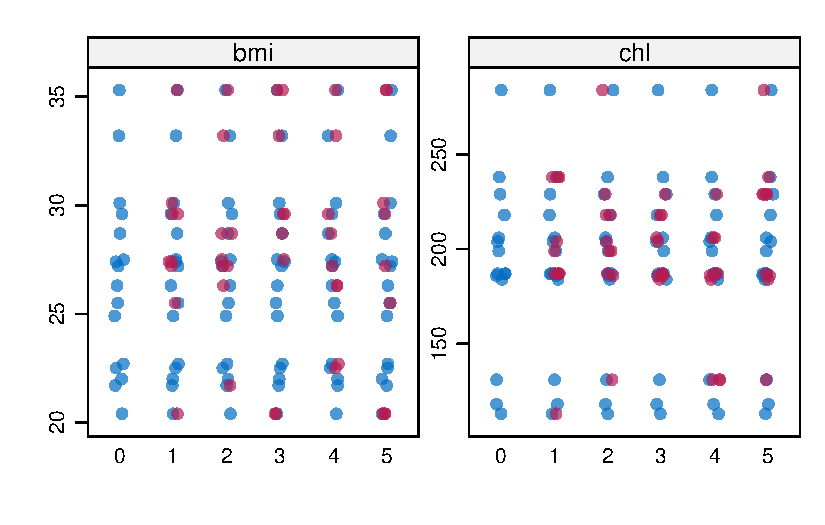
\includegraphics{guide_files/figure-pdf/unnamed-chunk-6-1.pdf}
\end{enumerate}

When you run this code you see how many imputed data sets you have. In
other words how many estimations you have for the missing values. This
is a harder topic to understand but in the code above it was specified
to impute 5 data sets which means we get five estimates for each missing
value. This allows us to pool this information in linear regression
which will be show later. We also see the summary of the methods used
for each variable. In the output we also get a graphs that compares the
values from the numerical variables that were imputed, bmi and chl. This
graph has for columns, 0 is the original data and 1 - 5 are each imputed
data set. The blue dots are the original data and the pink dots are the
imputed estimates. This graphs allows us to see how the estimates
compare to the original data. In our case we can see that the imputed
values fit very will with the original data and we do not see anything
that does not look realistic.

\begin{enumerate}
\def\labelenumi{\arabic{enumi}.}
\setcounter{enumi}{6}
\item
  The final step in our example is to fit a linear model with the data
  and pool across all imputed data sets to get a result. You can then
  compare the results of the pooled data vs the original data without
  missing values and see how you estimates would be different.

\begin{Shaded}
\begin{Highlighting}[]
\CommentTok{\# Analyze each imputed dataset and pool results (Example: Regression model)}
\NormalTok{fit }\OtherTok{\textless{}{-}} \FunctionTok{with}\NormalTok{(imp, }\FunctionTok{lm}\NormalTok{(bmi }\SpecialCharTok{\textasciitilde{}}\NormalTok{ age }\SpecialCharTok{+}\NormalTok{ hyp }\SpecialCharTok{+}\NormalTok{ chl))}
\NormalTok{pooled }\OtherTok{\textless{}{-}} \FunctionTok{pool}\NormalTok{(fit)}
\FunctionTok{summary}\NormalTok{(pooled)}
\end{Highlighting}
\end{Shaded}

\begin{verbatim}
         term    estimate  std.error  statistic        df      p.value
1 (Intercept) 18.46102980 3.86816817  4.7725510  9.946744 0.0007654584
2    age40-59 -6.49241684 2.41540227 -2.6879236  5.281569 0.0410531430
3    age60-99 -8.81689127 3.12353810 -2.8227257  4.219434 0.0448546454
4      hypyes  1.73190708 1.87962951  0.9214088 12.541653 0.3742218549
5         chl  0.06216513 0.02324192  2.6746982  7.498932 0.0298370851
\end{verbatim}
\end{enumerate}

The function with combines your imputed data with the linear model
example above. The pool function then pools across all imputed data sets
and gives you an average of all of your estimates, in our case 5. You
then have a linear model ``pool'' that you can summarize and compare
with our original data set with out imputation and missing values.

\begin{Shaded}
\begin{Highlighting}[]
\NormalTok{clean\_data }\OtherTok{\textless{}{-}} \FunctionTok{na.omit}\NormalTok{(nhanes2)}
\NormalTok{fit1 }\OtherTok{\textless{}{-}} \FunctionTok{lm}\NormalTok{(bmi }\SpecialCharTok{\textasciitilde{}}\NormalTok{ age }\SpecialCharTok{+}\NormalTok{ hyp }\SpecialCharTok{+}\NormalTok{ chl, clean\_data)}

\FunctionTok{summary}\NormalTok{(fit1)}
\end{Highlighting}
\end{Shaded}

\begin{verbatim}

Call:
lm(formula = bmi ~ age + hyp + chl, data = clean_data)

Residuals:
    Min      1Q  Median      3Q     Max 
-5.2752 -1.5329  0.0223  1.7676  4.2609 

Coefficients:
             Estimate Std. Error t value Pr(>|t|)   
(Intercept)  14.96300    4.26799   3.506  0.00801 **
age40-59     -6.61839    2.30156  -2.876  0.02065 * 
age60-99    -11.18114    3.36170  -3.326  0.01045 * 
hypyes        2.36161    2.53536   0.931  0.37886   
chl           0.07954    0.02445   3.253  0.01164 * 
---
Signif. codes:  0 '***' 0.001 '**' 0.01 '*' 0.05 '.' 0.1 ' ' 1

Residual standard error: 3.234 on 8 degrees of freedom
Multiple R-squared:  0.6697,    Adjusted R-squared:  0.5046 
F-statistic: 4.055 on 4 and 8 DF,  p-value: 0.04379
\end{verbatim}

From the two summary statements above you can see that you have a vast
difference in the estimates of the coefficients between fit1 without the
NA values and pooled with estimates for missing values. This allows you
to understand that estimating for missing values does have a major
impact on the model and in the end the conclusions that you make.

\section{Conclusion}\label{conclusion}

\bookmarksetup{startatroot}

\chapter*{References}\label{references}
\addcontentsline{toc}{chapter}{References}

\markboth{References}{References}

\phantomsection\label{refs}
\begin{CSLReferences}{1}{0}
\bibitem[\citeproctext]{ref-little2021}
Little, Roderick J. 2021. {``Missing Data Assumptions.''} \emph{Annual
Review of Statistics and Its Application} 8 (1): 89--107.
\url{https://doi.org/10.1146/annurev-statistics-040720-031104}.

\bibitem[\citeproctext]{ref-positpbcCreatingBook2024}
Posit PBC. 2024. {``Creating a Book. Quarto.''} July 1, 2024.
\url{https://quarto.org/docs/books/}.

\bibitem[\citeproctext]{ref-vanbuurenMiceMultivariateImputation2006}
Van Buuren, Stef, and Karin Groothuis-Oudshoorn. n.d. {``Mice:
Multivariate Imputation by Chained Equations.''}
\url{https://doi.org/10.32614/CRAN.package.mice}.

\end{CSLReferences}

\cleardoublepage
\phantomsection
\addcontentsline{toc}{part}{Appendices}
\appendix

\chapter{Topic}\label{topic}

Pick some subset of the information covered in your annual review
article that you are interested in exploring in more detail.

Identify the scope of your user guide - what will you cover? Specific
software packages? When to use or not to use a specific technique?

I will look into using likelihood methods for analyzing missing data, I
will cover how to use it and when to use it. I will attempt to discover
how to implement it in R. This will be done by showing a example of
using the mice package, found in R. This example will show the basics
and give a broad understanding of how to apply this package to a variety
of issues.

\chapter{Needs Assessment}\label{needs-assessment}

What does someone trying to accomplish your chosen task need help with?

\begin{itemize}
\tightlist
\item
  They will need help understanding why we need to estimate for missing
  values in our data set along with a method to use to properly estimate
  missing values. This will also mean they have to understand how and
  when to use the mice package in R and what methods to use for each
  variable.
\end{itemize}

What parts are likely to be tricky?

\begin{itemize}
\tightlist
\item
  Understanding the methods mathematically can be difficult as I do not
  fully understand the methods but implementing them in R is a task that
  can definitely be understood. This can be done with the mice package.
  I think a tricky element of this package can be understanding the
  prediction matrix along with what it is actually doing when the
  imputation is taking place.
\end{itemize}

What resources are already available on this topic that may be helpful?
Look for e.g.~software vignettes, package documentation, papers about
software packages, and so on.

\begin{itemize}
\tightlist
\item
  There is vignettes available which will be attached in a section in
  the user guide along with the references. We can see that there is
  also R documentation papers on this package which will also be
  attached.
\end{itemize}

\chapter{Task Analysis}\label{task-analysis}

Here are some questions to guide you through the process of doing a task
analysis. You don't have to specifically answer each one of these (and
some may not apply), but they should get you started thinking in the
right direction.

What are the prerequisites, for both knowledge and e.g.~software setup?

\begin{itemize}
\tightlist
\item
  The perquisites are understanding how to analyze data and run a linear
  model. Knowing what missing data is. Knowing basic statistical
  concepts not necessarily the mathematics behind it just how to apply
  it. The software needed to complete this task can be found in the R
  packages lattice and mice for the simple example in the user guide.
  There is other packages that the user may need but that will be on a
  case by case basis.
\end{itemize}

What are the basic requirements for any data that the method is used on?
Should the data be confined within a certain range? Does the data have
to be approximately normally distributed?

\begin{itemize}
\tightlist
\item
  The basic requirements is that the data has missing values as this is
  a imputation method to estimate missing values. We also know that the
  data can be of any form. The mice package has a wide range of methods
  that it used to estimate values which allows variety and flexibility
  in the type of data it uses.
\end{itemize}

What are the basic components of the task? Outline these in a bit more
detail.

\begin{itemize}
\item
  The data that you have needs to have missing values.
\item
  you need to have the mice package installed along with lattice ( the
  latter is more for imagery to compare).
\item
  Understand how prediction matrix and model selection works inside mice
  package.
\item
  Know how to use and implement lm() or glm() in R for creating linear
  and generalized linear models.
\end{itemize}

What decisions does the user need to be prepared to make on the fly?

\begin{itemize}
\tightlist
\item
  how to use the mice package in R
\item
  How to set up prediction matrix
\item
  How to select method of estimation
\item
  How to compare imputation data set to original data set
\end{itemize}

What questions should the user ask of the ``first draft'' of the
product? What adjustments may need to be made?

\begin{itemize}
\item
  I think the user will ask questions of how to apply this package a
  variety of problems that may not have been discussed in the user
  guide.
\item
  The user may also want to know more about the behind the scenes math
  that powers the package which this user will not be touching on.
\item
  Adjustments that may need to be made might be adding on to this user
  guide more examples for a variety of situations that may not be as
  common to see more specified cases of the mice package.
\end{itemize}

\section{Additional Guidance}\label{additional-guidance}

Your check-in should answer these basic questions (and similar concerns
that apply more directly to your topic).

Once you've completed the check-in, you can use this section to
jump-start an introduction/set-up/getting started section in your user
guide. This document should remain as an appendix to your main report.



\end{document}
